\chapter{Introduction}

\section{Cryptography vs. Cryptoanalysis}

Cryptography\index{Crypthography}: The constructive part (e.g. building systems, ``constructing the encryption''). \\
Cryptanalysis\index{Cryptanalysis}: The destructive part (e.g. breaking systems, ``cracking the code''). \\

This course covers both parts of Cryptology\index{Cryptology}. Both parts are needed in deployed systems, since we want to know how efficient the system is \textbf{and} how hard it is to break it:

\begin{example}
\ \\
\begin{itemize}
\item $2^{60}$ is inconvenient to compute, but totally doable;
\item $2^{70}$ is doable for academic clusters;
\item $2^{80}$ is doable for the NSA;
\item $2^{128}$ nobody can do that (including a security margin);
\end{itemize}
\end{example}

\begin{remark}
These numbers depend on the model of computation. Algorithms for example have different runtimes on quantum computers.
\end{remark}

%------------------------------------------------

\section{Caesar Cipher}\index{Caesar Cipher}

A standard example in cryptology is a \textsc{Caesar cipher}. In this example \textsc{Alice} (denoted \textsc{A} in figure \ref{fig:caesar_cipher}) wants to transmit a secret message ($E(m)$) to \textsc{Bob} (\textsc{B}), since the eavesdropper \textsc{Eve} (\textsc{E}) can see or hear everything on the channel.

\begin{figure}[H]
  \centering\import{Chapter1/Pictures/}{caesar_cipher.pdf_tex}
  \caption{Encrypted communication}
  \label{fig:caesar_cipher}
\end{figure}

So \textsc{Alice} and \textsc{Bob} decide to use a simple form of encryption - the \textsc{Caesars Cipher}. They replace the letters of the message by a letter some fixed number (in this case it is 3) of positions down the alphabet (see figure \ref{fig:caesar_cipher_ill}).

\begin{figure}[h]
\centering\includegraphics[scale=0.4]{Chapter1/Pictures/caesar_cipher_ill}
\caption{Idea of \textsc{Caesars Cipher}}
\label{fig:caesar_cipher_ill}
\end{figure}

\begin{example}
\ \\
The (original) message \\
 \textsc{HELLO} (Plaintext), 
 would be encrypted into \\
 \textsc{KHOOR} (Ciphertext)
\end{example}

This method of encryption is easy to cryptanalyze.

It is possible to turn this into a keyed encryption\index{Keyed Encryption}: $E_k(m)$, where the key $k$ gives the shifting distance. The decryption therefore is: $D_k(c)$, which should satisfy
\[
D_k(E_k(m)) = m.
\]

%------------------------------------------------

\section{Two types of crypto systems}

There are two types of crypto systems: \emph{symmetric} and \emph{asymmetric} (= public key) systems. In the \emph{symmetric} crypto \textsc{A} and \textsc{B} share the same key (e.g. the shifting distance of the \textsc{Caesars Cipher}, 128 bits in \textsc{AES}).

In \emph{public key} crypto each user has 2 keys:

\begin{itemize}
\item A \emph{public}\index{Public Key} one which can be used by anybody to encrypt messages to this user and
\item A \emph{private} (= secret key\index{Private Key}) one which the user uses to decrypt messages.
\end{itemize}

Therefore in \emph{asymmetric} systems this means $c= E_{P_k} (m), D_{S_k}(c) = m$, with $P_k$ the \emph{public key} and $S_k$ the \emph{secret key}. $P_k$ and $S_k$ can be of very different nature.

In a good crypto system one should not be able to recover $S_k$ from $P_k$ (= \emph{complete break}) or to decrypt $c$ without knowing $S_k$.

\begin{remark}
This means that there are two possiblities of cryptanalyzing a system. One can either find the \emph{secret key} or find the message. Obviously the first case means a \emph{complete break}, meaning that every other message can be decrypted as well.
\end{remark}

We will see different crypto systems such as \textsc{RSA}, \textsc{Elliptic-Curve Cryptography (ECC)} and \textsc{McEliece encryption} including attacks on these. \\

\noindent Crypto is also about authentication, e.g. digital signatures.

%TODO include Example of bank - asymmetric encryption

